% !TeX root = ../tfg.tex
% !TeX encoding = utf8

\chapter{Homología simplicial}
\label{chapter:homology}

Este capítulo se centra en la homología simplicial, una rama de estudio crucial
de la topología algebraica que utiliza complejos simpliciales para analizar y
comprender la estructura de espacios topológicos triangulables. Tras explorar los
fundamentos del álgebra homológica y la teoría de complejos simpliciales, ahora
profundizamos en las propiedades teóricas y aplicaciones prácticas de la
homología simplicial siguiendo los contenidos de \cite{rafael2003elementos}.

\section{Homología simplicial orientada}

Dado un símplice $\sigma$, podemos definir un orden sobre sus vértices. Dos
órdenes de $\sigma$ los consideraremos equivalentes si podemos pasar de uno a
otro con un número par de permutaciones. 
Además, en el caso donde $\sigma$ sea un $0$-símplice, claramente existe una única orientación.
Así, los ordenamientos posibles para
los vértices de $\sigma$ se pueden agrupar en dos clases de equivalencia
distintas, que definimos como las \textbf{orientaciones del símplice} $\sigma$.

\begin{definicion}
	Decimos que un símplice $\sigma = [a_{0}, a_{1}, \ldots, a_{p}]$ está \textbf{orientado}
	si se le ha asignado una de estas orientaciones. Utilizaremos $[a_{0}a_{1}\ldots
	a_{p}]$ para denotar la clase de equivalencia dada por la orientación $a_{0}< a
	_{1}< \cdots < a_{p}$ del símplice generado por los vértices $a_{0},a_{1},\ldots
	, a_{p}$.
\end{definicion}

Consideremos \(\Sigma_{p}\) el conjunto de todos los símplices de dimensión \(p\) de
un complejo simplicial geométrico \(K\) y el conjunto de sus clases de equivalencia por la relación de orientación. Para cada \(\sigma \in \Sigma_{p}\), definimos
\(\Sigma_{p}^{+}\) y \(\Sigma_{p}^{-}\) como los conjuntos que contienen, respectivamente,
un símplice orientado \(\sigma^{+}\) y el símplice con orientación opuesta
\(\sigma^{-}\). En lo que sigue, \(R\) siempre será un \textbf{anillo unitario conmutativo}, a menos que se indique de manera explícita lo contrario.

\begin{definicion}
	Sea \(K\) un complejo simplicial y sea \(R\) un anillo. Consideremos los conjuntos definidos anteriormente. Definimos el \textbf{\(R\)-módulo de las \(p\)-cadenas simpliciales orientadas}
	de \(K\), \(C_{p}(K;R)\), como el cociente del \(R\)-módulo libre generado por
	\(\Sigma_{p}^{+}\cup \Sigma_{p}^{-}\) sobre el submódulo generado por el
	conjunto \(\{\sigma^{+}+ \sigma^{-}: \sigma \in \Sigma_{p}\}\). Esto es,
	\[
	C_{p}(K;R) = \frac{R\langle \Sigma_{p}^{+}\cup \Sigma_{p}^{-}\rangle}{\langle
		\sigma^{+}+ \sigma^{-}: \sigma \in \Sigma_{p}\rangle}.
	\]
	Para \(p < 0\) o \(p > \dim(K)\), definimos \(C_{p}(K;R)\) como el \(R\)-módulo trivial.
\end{definicion}
El interés de definir el \(R\)-módulo de \(p\)-cadenas simpliciales orientadas radica
tanto en la identificación de los elementos que contiene como en las operaciones
algebraicas aplicables sobre ellos. Esta construcción nos permite manejar un
símplice orientado y su opuesto como opuestos algebraicos en un marco formal. Veámoslo.

Nuestro objetivo es demostrar que efectivamente
\[
\frac{R\langle \Sigma_{p}^{+}\cup \Sigma_{p}^{-}\rangle}{\langle \sigma^{+}+
	\sigma^{-}: \sigma \in \Sigma_{p}\rangle}\cong R \langle \tilde{\Sigma}_{p}\rangle
,
\]
donde \(\tilde{\Sigma}_{p}\) representa el conjunto de \(p\)-símplices en \(\Sigma_{p}\)
con una orientación arbitrariamente fija para cada uno.

Para ello, definamos la aplicación
\(f : \Sigma^{+}_{p}\cup \Sigma^{-}_{p}\to R \langle \tilde{\Sigma}_{p}\rangle\). Esta
aplicación asigna a cada símplice orientado \(\sigma^{+}\) en \(\Sigma_{p}^{+}\), un
representante \(\sigma\) en \(R \langle \tilde{\Sigma}_{p}\rangle\) con una
orientación fija elegida arbitrariamente, y a cada \(\sigma^{-}\) en \(\Sigma_{p}^{-}\),
le asigna \(-\sigma\) en \(R \langle \tilde{\Sigma}_{p}\rangle\), donde \(-\sigma\) refleja
el elemento opuesto de \(\sigma\).

La aplicación \(f\) respeta las relaciones de orientación al asignar a símplices con
orientaciones opuestas a elementos que son opuestos algebraicos en \(R \langle \tilde
{\Sigma}_{p}\rangle\). Por la \nameref{teo:univ-prop-free-mod}, esta aplicación
induce un homomorfismo
\(\tilde{f}: R\langle \Sigma_{p}^{+}\cup \Sigma_{p}^{-}\rangle \to R \langle \tilde
{\Sigma}_{p}\rangle\)
que resulta ser sobreyectivo, ya que cada elemento en \(R \langle \tilde{\Sigma}_{p}
\rangle\) tiene al menos una preimagen en \(R\langle \Sigma_{p}^{+}\cup \Sigma_{p}^{-}
\rangle\).

Por definición de \(f\), para cada elemento de la forma \(\sigma^{+}+ \sigma^{-}\)
en \(\langle \sigma^{+}+ \sigma^{-}: \sigma \in \Sigma_{p}\rangle\), tenemos que \(\tilde
{f}(\sigma^{+}+ \sigma^{-}) = f(\sigma^{+}) + f(\sigma^{-}) = \sigma - \sigma = 0\),
demostrando que todo el submódulo
\(\langle \sigma^{+}+ \sigma^{-}: \sigma \in \Sigma_{p}\rangle\) tiene imagen cero
por \(\tilde{f}\) y, por ende, está contenido en el núcleo de \(\tilde{f}\).

Además, si consideramos un elemento \(x\) en \(R\langle \Sigma_{p}^{+}\cup \Sigma_{p}
^{-}\rangle\) tal que \(\tilde{f}(x) = 0\), este elemento puede expresarse como una
combinación lineal de elementos en \(\Sigma_{p}^{+}\) y \(\Sigma_{p}^{-}\). La condición
\(\tilde{f}(x) = 0\) implica que la suma de las imágenes bajo \(f\) de los términos en
esta combinación lineal debe ser cero en \(R \langle \tilde{\Sigma}_{p}\rangle\).
Esto solo ocurre si para cada \(\sigma\), la suma total de los coeficientes correspondientes
a \(\sigma^{+}\) y \(\sigma^{-}\) es cero, lo que significa que cada término en \(x\)
que contribuye a esta suma cero debe ser de la forma \(\sigma^{+}+ \sigma^{-}\) o
un múltiplo de este, luego \(\tilde{f}(x) = 0\) implica que \(x \in \langle \sigma^{+}
+ \sigma^{-}: \sigma \in \Sigma_{p}\rangle\).

Por tanto, el núcleo de \(\tilde{f}\) coincide precisamente con
\(\langle \sigma^{+}+ \sigma^{-}: \sigma \in \Sigma_{p}\rangle\), y aplicando el \nameref{teo:first-iso},
concluimos que
\[
\frac{R\langle \Sigma_{p}^{+}\cup \Sigma_{p}^{-}\rangle}{\langle \sigma^{+}+
	\sigma^{-}: \sigma \in \Sigma_{p}\rangle}\cong R \langle \tilde{\Sigma}_{p}\rangle
,
\]
estableciendo la estructura algebraica deseada y completando la prueba.

\begin{observacion}
	En particular, la anterior construcción asigna a cada símplice orientado una
	cadena cuyo coeficiente del anillo es \(1\), \(0\) o \(-1\). A estas cadenas las
	llamaremos \textbf{\(p\)-cadenas elementales}. En ocasiones abusaremos de la
	notación para designar por \(\sigma\) a la cadena elemental respectiva del
	símplice orientado \(\sigma\).
\end{observacion}

\begin{definicion}
	Sea \(K\) un complejo simplicial y sean \(C_{p}(K;R), C_{p-1}(K;R)\) \(R\)-módulos de
	\(p\)-cadenas. Definimos el \textbf{operador borde de \(p\)-cadenas} como el homomorfismo
	\(\partial_{p}: C_{p}(K;R) \to C_{p-1}(K;R)\) tal que
	\[
	\partial_{p}(\sigma) = \partial_{p}([v_{0}, v_{1}, \ldots, v_{p}]) = \sum_{i=0}
	^{p}(-1)^{i}[v_{0}, \ldots, \hat{v}_{i}, \ldots, v_{p}] .
	\]
	donde \(\hat{v}_{i}\) denota el vértice a eliminar.
\end{definicion}
%Debemos verificar que \(\partial_p\) esté bien definido y que \(\partial_p(-\sigma) = -\partial_p \sigma\). Para este propósito, basta con mostrar que el lado derecho de (*) cambia de signo si intercambiamos dos vértices adyacentes en el arreglo \([v_0, \ldots, v_p]\). Así que comparemos las expresiones para
%\[
%\partial_p[v_0, \ldots, v_j, v_{j+1}, \ldots, v_p]
%\]
%y
%\[
%\partial_p[v_0, \ldots, v_{j+1}, v_j, \ldots, v_p].
%\]
%Para \(i \neq j, j+1\), los términos \(i\)-ésimos en estas dos expresiones difieren precisamente por un signo; los términos son idénticos excepto que \(v_j\) y \(v_{j+1}\) han sido intercambiados.
%
%¿Qué pasa con los términos \(i\)-ésimos para \(i = j\) y \(i = j + 1\)? En la primera expresión, uno tiene
%\[
%(-1)^j[\ldots, v_j, \hat{v}_{j}, v_{j+1}, \ldots] + (-1)^{j+1}[\ldots, v_j, v_{j+1}, \hat{v}_{j+1}, \ldots].
%\]
%En la segunda expresión, uno tiene
%\[
%(-1)^j[\ldots, v_{j+1}, \hat{v}_{j+1}, v_j, \ldots] + (-1)^{j+1}[\ldots, v_{j+1}, v_j, \hat{v}_j, \ldots].
%\]
%Comparando, se ve que estas dos expresiones difieren por un signo.
\begin{lema}
	El operador borde \(\partial_{p}: C_{p}(K;R) \to C_{p-1}(K;R)\) está bien definido.
	En particular, si \(\sigma^{+}\) y \(\sigma^{-}\) son las dos orientaciones del \(p\)-símplice
	\(\sigma\), tenemos que
	\[
	\partial_{p}(\sigma^{+}+\sigma^{-}) = 0
	\]
\end{lema}
\begin{proof}
	Probaremos que la suma de la imagen por el operador borde de \(\sigma^{+}= [v_{0}
	v_{1}\ldots v_{p}]\) y \(\sigma^{-}= [v_{1}v_{0}\ldots v_{p}]\) es igual a \(0\).
	Para ello, observamos que
	\begin{align*}
		\partial_{p}\sigma^{+} & = [v_{1}v_{2}\ldots] - [v_{0}v_{2}\ldots] + \sum_{i\ne0,1}(-1)^{i}[v_{0}v_{1}\ldots \hat{v}_{i}\ldots v_{p}], \\
		\partial_{p}\sigma^{-} & = [v_{0}v_{2}\ldots] - [v_{1}v_{2}\ldots] + \sum_{i\ne0,1}(-1)^{i}[v_{1}v_{0}\ldots \hat{v}_{i}\ldots v_{p}].
	\end{align*}
	Al sumar ambas expresiones, los dos primeros términos de
	\(\partial_{p}\sigma^{+}\) y \(\partial_{p}\sigma^{-}\) se cancelan entre sí. Como
	consecuencia de la definición de \(C_{p-1}(K;R)\), los términos restantes
	definen orientaciones opuestas del mismo símplice por lo que se cancelan y
	\(\partial_{p}(\sigma^{+}+\sigma^{-})=0\).
\end{proof}

\begin{lema}
	Sean \(\partial_{p}: C_{p+1}(K;R) \to C_{p}(K;R)\),
	\(\partial_{p}: C_{p}(K;R) \to C_{p-1}(K;R)\) operadores borde. Entonces \(\partial
	_{p}\circ \partial_{p+1}= 0\).
\end{lema}
\begin{proof}
	\begin{gather*}
		\partial_{p}\partial_{p+1}[v_{0}, \ldots, v_{p+1}] = \partial_{p}\left( \sum_{i=0}
		^{p+1}(-1)^{i}[v_{0}\ldots \hat{v}_{i}\ldots v_{p+1}] \right) \\ = \sum_{i=0}
		^{p+1}(-1)^{i}\left[ \sum_{j>i}^{p+1}(-1)^{j}[v_{0}\ldots, \hat{v}_{i}\ldots
		\hat{v}_{j}\ldots v_{p+1}] + \sum_{j=0}^{j<i}(-1)^{j}[v_{0}\ldots \hat{v}_{j}
		\ldots \hat{v}_{i}\ldots v_{p+1}] \right].
	\end{gather*}
	Es decir, el símplice
	\([v_{0}\ldots,\hat{v}_{k}\ldots,\hat{v}_{t}\ldots, v_{p+1}]\) aparece dos veces
	en la anterior expresión con signos opuestos, donde \(k,t \in \{0, \ldots, p+1\}\).
	Esto nos lleva a discutir los siguientes casos. Supongamos sin pérdida de generalidad
	que \(k < t\). En el primer caso, \(i = k < j = t\) donde el coeficiente es \((-1)^{k}
	(-1)^{t-1}\). En el segundo caso, \(i = t > j = k\) con coeficiente \((-1)^{t}(-1)^{k}\).
	Concluimos por tanto que todo símplice de la expresión se anula y al anularse
	sobre los generadores, \(\partial_{p-1}\partial_{p}\) es el homomorfismo nulo.
\end{proof}

\begin{definicion}
	El complejo de cadenas positivo \(C_{\bullet}(K;R) = \{C_{p}(K;R), \partial_{p}\}\)
	lo llamaremos \textbf{complejo de cadenas simpliciales} de \(K\). La homología de
	dicho complejo la notaremos por \(H_{p}(K;R)\) y lo llamaremos \textbf{\(p\)-ésimo
		\(R\)-módulo de homología} de \(K\).
\end{definicion}
Si \(R=\Z\), el módulo \(H_{p}(K;\Z)\) lo notaremos simplemente por \(H_{p}(K)\) y diremos
que es el \textbf{\(p\)-ésimo grupo de homología} de \(K\).

\begin{proposicion}
	\label{prop:aumento} Sea \(K\) un complejo simplicial no vacío. Entonces el
	complejo de cadenas positivo \(\{ C_{p}(K;R), \partial_{p}\}\) admite un aumento.
\end{proposicion}
\begin{proof}
	Sea \(\varepsilon: C_{0}(K;R) \to R\) el homomorfismo que extiende linealmente \(\varepsilon
	(v) = 1\) para todo vértice \(v \in K\). Veamos que
	\(\varepsilon \circ \partial_{1}: C_{1}(K;R) \to R\) es nulo. Tomando \([v_{0},v_{1}
	] \in C_{1}(K;R)\) obtenemos que \(\varepsilon (\partial_{1}[v_{0},v_{1}]) = \varepsilon
	(v_{1}- v_{0}) = 1-1 = 0\), como queríamos ver.
\end{proof}

\begin{definicion}
	Sea \(\widetilde{C}_{\bullet}(K;R)\) el complejo aumentado del complejo de cadenas
	simpliciales \(C_{\bullet}(K;R)\). Denominaremos \textbf{\(p\)-ésimo módulo de
		homología reducida} de \(K\) al módulo de homología \(H_{p}(\widetilde{C}_{\bullet}
	;R)\) y lo denotaremos por \(\widetilde{H}(K;R)\).
\end{definicion}

\begin{proposicion}
	\label{prop:simpl_app_hom} Sean \(K\) y \(L\) dos complejos simpliciales junto con
	una aplicación simplicial \(f: |K| \to |L|\). Esta aplicación induce un
	homomorfismo entre los complejos de cadenas, \(C(f)\), el cual se define
	extendiendo linealmente la función
	\[
	C(f)([v_{0}\ldots v_{p}]) =
	\begin{cases}
		[f(v_{0}) \ldots f(v_{p})] & \text{si los vértices son distintos entre sí}, \\
		0                          & \text{en caso contrario}.
	\end{cases}
	\]
	En particular, si \(f\) es la identidad, entonces \(C(f)\) es simplemente la
	identidad también. Además, si \(g: |L| \longrightarrow |M|\) es otra aplicación
	simplicial, se cumple que \(C(g \circ f) = C(g) \circ C(f)\).
\end{proposicion}
\begin{proof}
	Para demostrar esto, primero observamos que la definición de \(C(f)\) es
	independiente de la orientación de los símplices. Luego, verificamos la
	igualdad \(\partial_{p}\circ C(f) = C(f) \circ \partial_{p}\). Si no hay vértices
	repetidos, se tiene que:
	\begin{gather*}
		C(f) \partial_{p}([v_{0}\ldots v_{p}]) = C(f) \left( \sum_{i=0}^{p}(-1)^{i}[v
		_{0}\ldots \hat{v}_{i}\ldots v_{p}] \right) = \\ \sum_{i=0}^{p}(-1)^{i}[f(v_{0}
		) \ldots \widehat{f(v_i)}\ldots f(v_{p})] = \partial_{p}C(f)([v_{0}\ldots v_{p}
		]).
	\end{gather*}
	Si hay vértices repetidos, digamos \(f(v_{i}) = f(v_{j})\), entonces \(\partial_{p}
	C(f)([v_{0}\ldots v_{p}]) = 0\). Por otro lado,
	\[
	\sum_{i=0}^{p}(-1)^{i}C(f)([v_{0}\ldots \hat{v_i}\ldots v_{p}]) = 0
	\]
	debido a que \(C(f)([v_{0}\ldots \hat{v}_{k}\ldots v_{p}]) = 0\) para \(k \neq i,j\)
	y cuando \(i < j\),
	\[
	(-1)^{i}[f(v_{0}) \ldots \widehat{f(v_i)}\ldots f(v_{j}) \ldots f(v_{p})] + (
	-1)^{j}[f(v_{0}) \ldots f(v_{i}) \ldots \widehat{f(v_j)}\ldots f(v_{p})] = 0
	\]
	también se anula. Esto se debe a que si no hay más vértices repetidos, como
	\(f(v_{i}) = f(v_{j})\), el número de trasposiciones necesarias para cambiar de un
	símplice orientado al otro es \(j-i-1\), dado que \(f(v_{j})\) ocupa el lugar
	\(j-1\) en el primer símplice. La fórmula \(C(g \circ f)=C(g)C(f)\) se sigue directamente
	de la definición de \(C(f)\).
\end{proof}
\begin{observacion}
	El resultado anterior nos garantiza que \(C: \Cat{Csim}\to R \textbf{-}\Cat{Ch_\bullet}\)
	es un funtor covariante entre la categoría de complejos simpliciales y la categoría
	de complejos de cadenas.
\end{observacion}

\begin{definicion}
	\label{def:chain-map-ind} Sea \(f : |K| \to |L|\) una aplicación simplicial y sea
	\(C(f): C_{\bullet}(K;R) \to C_{\bullet}(L;R)\) una aplicación de cadenas definida
	como en la \autoref{prop:simpl_app_hom}. Llamaremos a \(C(f)\) la \textbf{aplicación
		de cadenas inducida por} \(f\) y la notaremos por \(f_{\#}\).
\end{definicion}

\begin{corolario}
	Toda aplicación simplicial inducida \(f: |K| \to |L|\) induce un homomorfismo de
	\(R\)-módulos
	\[
	H_{p}(f) : H_{p}(K;R) \to H_{p}(L;R)
	\]
	que notaremos por \(f_{*}\) y que cumple que si \(g: |L| \to |M|\) es otra aplicación
	simplicial, entonces \((g \circ f)_{*}= g_{*}\circ f_{*}\) e \(\id_{*}= \id\).
\end{corolario}
\begin{observacion}
	La última implicación del corolario se traduce en que tenemos un funtor covariante
	que va de la categoría de complejos simpliciales con los homeomorfismos simpliciales
	a la categoría de \(R\)-módulos con sus homomorfismos.
\end{observacion}

\begin{lema}
	La aplicación de cadenas \(f_{\#}: C_{\bullet}(K;R) \to C_{\bullet}(L;R)\) preserva
	el homomorfismo de aumento y como resultado, induce un homomorfismo \(f_{*}\) de
	módulos de homología reducida.
\end{lema}
\begin{proof}
	Sea \(f : |K| \to |L|\) una aplicación simplicial, \(f_{\#}\) su aplicación de
	cadenas inducida y sean
	\(\varepsilon : C_{0}(K;R) \to R,\ \varepsilon : C_{0}(L;R) \to R\) aumentos de
	\(C_{\bullet}(K;R), C_{\bullet}(L;R)\) respectivamente. Llamemos indistintamente
	\(\varepsilon\) a ambos aumentos en función del dominio en el que nos encontremos.
	Ahora definamos \(\varepsilon (f_{\#}(v)) = 1\) y \(\varepsilon(v) = 1\) para todo
	vértice de \(K\) y extendamos por linealidad. Por consiguiente \(\varepsilon \circ
	f_{\#}= \varepsilon\). Esta ecuación implica que \(f_{\#}\) lleva el núcleo de
	\(\varepsilon_{K}: C_{0}(K;R) \to R\) al núcleo de
	\(\varepsilon_{L}: C_{0}(L;R) \to R\), lo que induce un homomorfismo \(f_{*}: \widetilde
	{H}_{0}(K;R) \to \widetilde{H}_{0}(L;R)\).
\end{proof}
\begin{teorema}
	Sean \(f, g\) aplicaciones simpliciales de \(K\) a \(L\); \(f_{\#}, g_{\#}\) sus
	aplicaciones de cadenas inducidas y sea \(s: f_{\#}\to g_{\#}\) una homotopía de
	cadenas entre ellas. Entonces los homomorfismos inducidos \(f_{*}, g_{*}\) para sus
	módulos de homología son iguales.
\end{teorema}
\begin{proof}
	Sea \(z\) un \(p\)-ciclo de \(K\). Entonces
	\[
	g_{*}(z) - f_{*}(z) = \partial sz + s\partial z = \partial sz + 0
	\]
	por lo que \(f(z)\) y \(g(z)\) tienen la misma clase de homología. Por tanto,
	\(f_{*}([z]) = g_{*}([z])\) como se quería.
\end{proof}
%
%El siguiente teorema muestra una propiedad esencial de los módulos de homología: el módulo \(H_0(K;R)\) indica el número de componentes conexas de \(K\).
%\begin{teorema}
%	Dado un complejo simplicial \( K \), se tiene que \( H_0(K) \) es un grupo abeliano libre. Además, si \( \{v_\alpha\} \) es una colección de vértices con un elemento \( v_\alpha \) por cada componente conexa de \( |K| \), entonces las clases de homología de los \( v_\alpha \) forman una base de \( H_0(K) \).
%\end{teorema}
%\begin{proof}
%	Seguiremos en un principio la demostración propuesta en el [10, Teorema 7.1], dividiendo la prueba en varios pasos:
%
%	\textbf{PASO 1.} Comenzamos estableciendo una relación de equivalencia entre vértices \(u\) y \(v\) de \(K\), definida por la existencia de una secuencia finita de vértices \(u = a_0, a_1, \ldots, a_n = v\), donde cada par \((a_{i-1}, a_i)\) forma un 1-símplice en \(K\). Denotemos por \(C_v\) la unión de las estrellas de todos los vértices \(u\) que están relacionados con \(v\), esto es,
%	\[ C_v = \bigcup_{u \sim v} St(u), \]
%	donde \(St(u)\) es la unión de los interiores de todas las caras de \(K\) que contienen a \(u\). Esta construcción garantiza que cada \(C_v\) es abierto, ya que cada \(St(u)\) es un abierto en \(|K|\), y además cada \(C_v\) es conexo por caminos, lo cual se deriva de la posibilidad de trazar caminos a través de las secuencias de 1-símplices que definen la relación de equivalencia. Así, cada \(C_v\) corresponde a una componente conexa de \(|K|\).
%
%	Veamos que las \( C_v \) se corresponden con las componentes conexas de \( |K| \):
%
%	\begin{itemize}
	%		\item Los \( C_v \) son abiertos en \( K \) porque \( St(u) \) es abierto en \( |K| \).
	%		\item Cada \( C_v \) es conexo por caminos y por consiguiente conexo ([20, Teorema 2.7]).
	%	\end{itemize}
%
%	Dado un vértice \( u \), sea \( u \sim v \) y \( x \in St(u) \). Por definición de la relación de equivalencia, existen vértices \( u = a_0, a_1, \ldots, a_n = v \) que cumple la condición antes enunciada. Son precisamente los 1-símplices \( [a_0, a_1], \ldots, [a_{n-1}, a_n] \) los que garantizan la existencia de un camino entre \( u \) y \( v \). Por su parte, como camino entre \( u \) y \( z \) basta tomar la recta que une ambos puntos, la cual estará contenida en \( K \) debido al carácter afín de un símplice presentado en la Definición 1.2.
%
%	Si \( C_u \neq C_v \) entonces \( C_u \cap C_v \) será vacío. Supongamos que existe un \( x \in C_u \cap C_v \). Entonces
%	\[ x \in St(u) \cap St(u'), \]
%	con \( u \sim v \) y \( u' \sim v' \). Si \( u = u' \), entonces \( u \sim v \) es \( u' \sim v' \), lo cual resulta una contradicción. Por el contrario, si \( u \neq u' \), tenemos que existe una cara \( A \) con \( u \) como vértice que contiene a \( x \) en su interior y que existe una cara \( B \) con \( u' \) como vértice que contiene a \( x \) en su interior. Supongamos que la dimensión de \( A \) es menor o igual que la de \( B \). Entonces, como la intersección de dos caras es una cara y \( x \) pertenece al interior de \( A \), tenemos que \( A \subseteq B \), y por tanto el 1-símplice \( [u,u'] \) está en \( K \). En consecuencia, \( u \sim v \) o \( u' \sim v' \), lo cual nos lleva a una contradicción.
%
%	\textbf{PASO 2.} Sea \( w \) una colección de vértices de \( K \) con \( v_\alpha \in C_\alpha \). Sea \( w \) un vértice de \( K \). Se tendrá \( w \in C_\alpha \) para algún \( \alpha \). Por definición, existe una sucesión de vértices \( v_\alpha = a_0, a_1, \ldots, a_n = w \) tal que los 1-símplices \( [a_i, a_{i+1}] \) están en \( K \). Consideremos la 1-cadena
%	\[ c = [a_0, a_1] + [a_1, a_2] + \ldots + [a_{n-1}, a_n] . \]
%
%	Se tiene
%	\[ \partial c = a_n - a_0 = w - v_\alpha , \]
%	con lo cual la cadena \( w \) es homóloga a la cadena \( v_\alpha \). De este modo, cualquier 0-cadena en \( K \) es homóloga a una cadena de la forma \( \sum n_\alpha v_\alpha \).
%
%	Llegados a este punto, para ver que las clases de homología de los \( v_\alpha \) forman una base de \( H_0(K) \), tenemos que ver el siguiente y último paso de la demostración.
%
%	\textbf{PASO 3.} Veamos que una 0-cadena de la forma \( c = \sum n_\alpha v_\alpha \) es borde si y solo si \( n_\alpha = 0 \) para todo \( \alpha \).
%
%	Supongamos para ello que \( c = \partial d \). Podemos expresar la 2-cadena \( d \) como una sumatoria de 1-cadenas donde cada sumando tiene soporte en una componente conexa de \( K \). Es decir, \( d = \sum d_\alpha \), donde cada \( d_\alpha \) tiene soporte en \( C_\alpha \). De este modo, \( \partial d = \sum \partial d_\alpha \), donde \( \partial d_\alpha \) es una 0-cadena soportada por \( C_\alpha \). Por la definición de \( C_0(K) \) como módulo libre, esto implica que \( \partial d_\alpha = n_\alpha v_\alpha \) para todo \( \alpha \).
%
%	Veamos ahora que esto implica que \( n_\alpha = 0 \):
%
%	Definimos la aplicación
%	\[ \varepsilon : C_0(K) \rightarrow \mathbb{Z}, \quad c = \sum m_\alpha v_\alpha \mapsto \sum m_\alpha . \]
%	(Si construimos nuestras cadenas sobre otro módulo la definición de esta aplicación no cambia, solo variará el rango de la misma). En particular tenemos que
%	\[ \varepsilon(\partial[w, v]) = \varepsilon(w - v) = \varepsilon(w) - \varepsilon(v) = 0 , \]
%	de donde se deduce que \( \varepsilon(\partial d_\alpha) = 0 \), lo cual nos lleva a que
%	\[ n_\alpha = \varepsilon(n_\alpha v_\alpha) = \varepsilon(\partial d_\alpha) = 0 , \]
%	tal y como queríamos demostrar.
%\end{proof}

\section{Homología del complejo cono}
A continuación, exploraremos un nuevo complejo simplicial que construiremos a partir
de otro dado. El complejo cono nos facilitará la obtención de algunos resultados
relevantes en homología.
\begin{definicion}
	Sea \(K\) un complejo simplicial de \(\R^{N}\) y sea \(w \in \R^{N}\) tal que cada semirrecta
	con origen \(w\) corta a \(|K|\) a lo sumo en un punto. Definimos el \textbf{cono
		sobre \(K\) con vértice \(w\)} como el conjunto cuyos elementos son los símplices de
	\(K\) o símplices de la forma \([w,v_{0},\ldots,v_{p}]\), donde
	\([v_{0}, \ldots, v_{p}] \in K\). Lo denotaremos por \(w \ast K\).
\end{definicion}

\begin{figure}[h]
	\centering % This centers the figure
	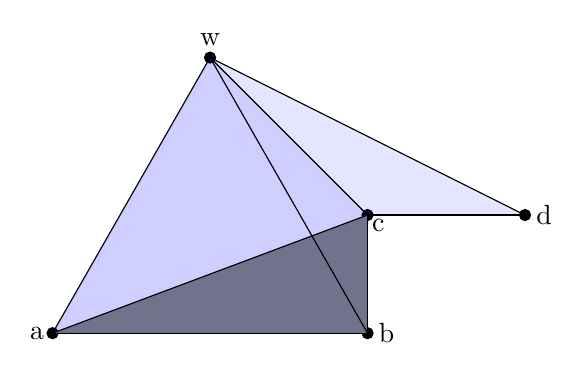
\begin{tikzpicture}
		% Define the style for the nodes
		\tikzstyle{every node}
		=[circle, draw, fill=black, inner sep=0pt, minimum width=4pt]
		
		% Nodes definition with labels
		\node (a) at (-2, 0) [label=left:a] {}; \node (b) at (2, 0) [label=right:b] {};
		\node (w) at (0, 3.5) [label=above:w] {}; \node (c) at (2, 1.5) [label=below right:c]
		{}; \node (d) at (4, 1.5) [label=right:d] {};
		
		% Draw the gray-filled area
		\fill[gray] (a.center) -- (b.center) -- (c.center) -- cycle;
		
		% Draw the translucent light blue-filled areas
		\filldraw[fill=blue, opacity=0.1] (a.center) -- (w.center) -- (c.center) --
		cycle; \filldraw[fill=blue, opacity=0.1] (b.center) -- (w.center) -- (c.center)
		-- cycle; \filldraw[fill=blue, opacity=0.1] (a.center) -- (w.center) -- (b.center)
		-- cycle; \filldraw[fill=blue, opacity=0.1] (c.center) -- (d.center) -- (w.center)
		-- cycle;
		
		% Draw the tetrahedron edges
		\draw (a.center) -- (b.center); \draw (b.center) -- (w.center); \draw (w.center)
		-- (a.center); \draw (a.center) -- (c.center); \draw (b.center) -- (c.center);
		\draw (w.center) -- (c.center); \draw (c.center) -- (d.center); \draw (w.center) -- (d.center); 
	\end{tikzpicture}
	\caption{Cono sobre el complejo formado por el \(2\)-símplice \([a,b,c]\), el $1$-símplice $[c,d]$ y todas sus caras con vértice \(w\).}
\end{figure}

\begin{lema}
	El cono \(w \ast K\) es un complejo simplicial.
\end{lema}
\begin{proof}
	Sea \(\sigma = [v_{0},\ldots,v_{p}]\) un símplice de \(K\). Primero veamos que el
	conjunto \(\{w,v_{0},\ldots,v_{p}\}\) es afínmente independiente. Si \(w\) perteneciera
	al plano \(P\) generado por los puntos \(v_{0},\ldots,v_{p}\), podríamos
	considerar el segmento que une \(w\) con un punto de \(x \in \interior \sigma\). Dicho
	conjunto, por ser abierto en \(P\), contendría un intervalo de puntos en el segmento,
	contradiciendo la hipótesis de que las semirrectas que parten de \(w\) cortan a
	lo sumo en un punto a \(|K|\).
	
	Veamos ahora que \(w \ast K\) es un complejo simplicial. Los símplices de \(w \ast
	K\) pueden ser de tres tipos:
	\begin{enumerate}
		\item Símplices \([v_{0},\ldots, v_{p}]\) pertenecientes a \(K\).
		
		\item Símplices de la forma \([w,v_{0},\ldots, v_{p}]\).
		
		\item El \(0\)-símplice \([w]\).
	\end{enumerate}
	Si \(\sigma,\tau\) son símplices del primer tipo, entonces \(\interior \sigma \cap
	\interior \tau = \emptyset\) puesto que \(K\) es un complejo simplicial. El
	símplice \(\interior [w,v_{0},\ldots,v_{p}]\) es la unión de todos los segmentos
	abiertos que unen \(w\) con \(v_{0},\ldots, v_{p}\), luego dos símplices de esta forma
	tienen intersección vacía pues las semirrectas que parten de \(w\) cortan a \(K\) a
	lo sumo en un punto. Finalmente, si \(\sigma\) es del primer tipo y \(\tau\) del segundo,
	\(\interior \sigma \cap \interior \tau = \emptyset\) por el mismo argumento
	recién dado.
\end{proof}

\begin{proposicion}
	\label{prop:char-homol-cono} Sea \(K\) un complejo simplicial y sea \(w \ast K\) el
	cono sobre \(K\) de vértice \(w\). Entonces la homología orientada de \(w \ast K\)
	es \(H_{p}(w \ast K;R) = 0\) para todo \(p \neq 0\) y \(H_{0}(w \ast K;R) \cong R\).
	En el caso de la homología reducida, \(\widetilde{H}_{0}(w \ast K;R) = 0\) para
	todo \(p \in \Z\).
\end{proposicion}
\begin{proof}
	Sea \(D_{\bullet}= \{D_{p}, \partial_{p}\}\) un complejo de cadenas tal que \(D_{p}
	= 0\) para todo \(p \neq 0\) y \(D_{0}= R\). Definimos la aplicación de cadenas
	\(f: D_{\bullet}\to C_{\bullet}(w \ast K;R)\) de forma que \(f_{p}= 0\) para todo
	\(p \neq 0\) y \(f_{0}(r)=rw\). Por otro lado, por la \autoref{prop:aumento}
	podemos definir el aumento
	\(\varepsilon: C_{\bullet}(w \ast K;R) \to D_{\bullet}\) dado por
	\(\varepsilon_{p}=0\) para todo \(p \neq 0\) y \(\varepsilon_{0}(v) = 1\) para todo
	vértice \(v\) del cono. Nuestro objetivo es ver que efectivamente \(f\) es una equivalencia
	de cadenas junto a \(\varepsilon\). De manera directa tenemos que
	\(\varepsilon \circ f = \id_{D}\), luego \(\varepsilon \circ f \simeq \id_{D}\).
	Veamos ahora que \(f \circ \varepsilon\) es homotópica a la identidad. Para ello
	vamos a definir \(s\) como la familia \(\{s_{p}\}\) de homomorfismos \(s_{p}: C_{p}(
	w \ast K;R) \to C_{p+1}(w \ast K;R)\) tal que
	\[
	s_{p}([v_{0}\ldots v_{p}]) =
	\begin{cases}
		[wv_{0}\ldots v_{p}] \  & \text{si}\ v_{i}\neq w \quad 0 \leq i \leq p,\quad p \geq 0, \\
		0 \                     & \text{en caso contrario},
	\end{cases}
	\]
	induce una extensión lineal. Dicha familia está bien definida para
	\(C_{p}(w \ast K;R)\). Veamos que \(\partial_{p+1}s_{p}+ s_{p-1}\partial_{p}= \id_{C_p(w
		\ast K;R)}- f_{p}\varepsilon_{p}\) se cumple, por lo que \(s\) es una homotopía
	de cadenas. Para el caso en que \(p \in \Z\) es menor que \(0\), se cumple de manera
	trivial. Si \(p = 0\), distinguimos dos casos. Cuando \(v \neq w\) tenemos que \((\partial
	_{1}s_{0}+s_{-1}\partial_{0})(v) = \partial_{1}[w,v] = v-w = (\id_{0}- f_{0}\varepsilon
	_{0})(v)\). Por el contrario si \(v = w\), \((\partial_{1}s_{0}+s_{-1}\partial_{0})
	(v) = 0\) y también \((\id_{0}- f_{0}\varepsilon_{0})(v) = \id_{0}(w) - (f_{0}\varepsilon
	_{0})(w) = w - w = 0\). Por último, veamos que sucede cuando \(p > 0\).
	Supongamos primero que \(w \neq v_{i}\). Entonces
	\begin{gather*}
		(\partial_{p+1}s_{p}+ s_{p-1}\partial_{p})[v_{0}\ldots v_{p}] =\partial_{p+1}
		[wv_{0}\ldots v_{p}]+s_{p-1}\left(\sum_{i=0}^{p}(-1)^{i}[v_{0}\ldots\hat{v}_{i}
		\ldots v_{p}]\right) \\ =[v_{0}\ldots v_{p}]+\sum_{i=0}^{p}(-1)^{i+1}[wv_{0}\ldots
		\hat{v}_{i}\ldots v_{p}]+\sum_{i=0}^{p}(-1)^{i}[wv_{0}\ldots\hat{v}_{i}\ldots
		v_{p}] \\ =[v_{0}\ldots v_{p}]=(id_{C_{p}}-f_{p}\varepsilon_{p})[v_{0}\ldots
		v_{p}].
	\end{gather*}
	Finalmente si \(w = v_{i_0}\) para algún \(i_{0}\) entonces
	\begin{gather*}
		(\partial_{p+1}s_{p}+s_{p-1}\partial_{p})[v_{0}\ldots v_{p}]=s_{p-1}\partial_{p}
		[v_{0}\ldots v_{p}] =s_{p-1}\left( \sum_{i=0}^{p-1}(-1)^{i}[v_{0}\ldots \hat{v}
		_{i}\ldots v_{p}] \right) \\ =(-1)^{i_0}s_{p-1}[v_{0}\ldots \hat{v}_{i_0}\ldots
		v_{p}] =(-1)^{i_0}[wv_{0}\ldots \hat{v}_{i_0}\ldots v_{p}] \\ =(-1)^{i_0}[v_{i_0}
		v_{0}\ldots \hat{v}_{i_0}\ldots v_{p}] =[v_{0}\ldots v_{p}].
	\end{gather*}
	Es decir, \(f \circ \varepsilon \simeq \id_{C(w \ast K;R)}\) y por el
	\autoref{cor:equiv-homot} induce un isomorfismo
	\(\varepsilon_{*}: H_{p}(w \ast K;R) \to H_{p}(D;R)\).
	
	Para el caso reducido consideremos el complejo aumentado \(D_{\bullet}\) dado
	por el aumento \(\id_{R}: D_{0}\to R\). Como consecuencia, la homología de
	\(\widetilde{D}\) es trivial. Además, podemos extender los homomorfismos
	\(\varepsilon\) y \(f\) a homomorfismos \(\widetilde{\varepsilon}\) y
	\(\widetilde{f}\) para los complejos aumentados de forma que
	\(\widetilde{\varepsilon}_{-1}= \widetilde{f}_{-1}= \id_{R}\). Por la misma homotopía
	\(s\) obtenemos que \(\widetilde{\varepsilon}\) y \(\widetilde{f}\) son equivalencias
	homotópicas entre los complejos aumentados y por tanto,
	\(\widetilde{H}_{p}(w \ast K;R) = 0\) para todo \(p \in \Z\).
\end{proof}
\begin{corolario}
	\label{cor:cono-nulo} La homología simplicial reducida de cualquier símplice es
	nula.
\end{corolario}
\begin{corolario}
	Sea \(\sigma\) un \(n\)-símplice y sea \(\bd \sigma\) su borde. Entonces
	\(\widetilde{H}_{p}(\bd \sigma;R) = 0\) es trivial si \(p \neq n-1\) y
	\(\widetilde{H}_{n-1}(\bd \sigma; R) \cong R\). Además, para el caso no trivial,
	un generador es la clase de la cadena \(\partial(\sigma)\).
\end{corolario}
\begin{proof}
	Dado el símplice anterior, los complejos de cadenas aumentados de \(\sigma\) y
	su borde coinciden hasta dimensión \(p \leq n-1\). Por el \autoref{cor:cono-nulo}
	deducimos que \(\widetilde{H}_{p}(\bd \sigma; R) = 0\) para \(p \leq n-2\). Además,
	\(C_{p}(\bd \sigma; R) = 0\) para \(p \geq n\). Por lo tanto, \(\widetilde{H}_{n-1}(
	\bd\sigma;R)=\ker \partial_{n-1}\). Aquí, \(\partial_{n-1}\) representa el operador
	borde en ambos complejos aumentados (es decir, \(\partial_{0}=\varepsilon\) indica
	el aumento). Dado que el complejo aumentado de \(\sigma\) tiene homología trivial,
	entonces \(\ker \partial_{n-1}=\im, \partial_{n}\), y además \(\partial_{n}\) es inyectivo
	donde el operador borde \(\partial_{n}: C_{n}(\sigma; R) \rightarrow C_{n-1}(\sigma
	; R) = C_{n-1}(\bd \sigma; R)\) aparece en el complejo de \(\sigma\). Puesto que
	\(C_{n}(\sigma;R)\) es isomorfo a \(R\) generado por \(\sigma\), se sigue que \(\im \partial
	_{n}\), y por tanto \(\widetilde{H}_{n-1}(\bd\sigma;R)\), es isomorfo a \(R\) generado
	por \(\partial(\sigma)\).
\end{proof}

\section{Sucesión de Mayer-Vietoris}
Nombrada en honor a los matemáticos austriacos Walther Mayer y Leopold Vietoris,
la sucesión de Mayer-Vietoris es una herramienta esencial en la topología algebraica
y la teoría de homología. Esta sucesión permite analizar la homología de un
complejo simplicial a partir de la homología de sus subcomplejos, de manera análoga
a como el teorema de Seifert-van Kampen describe el grupo fundamental de un espacio
topológico a partir de subespacios abiertos y conexos por arcos.
\begin{lema}
	[Lema de la serpiente] \label{lem:zig-zag} Sean \(A_{\bullet}= \{A_{n},\partial_{A}
	\}, B_{\bullet}= \{B_{n},\partial_{A}\}\) y \(C_{\bullet}= \{C_{n},\partial_{C}\}\)
	complejos de cadenas y sean \(f,g\) aplicaciones de cadenas tales que la sucesión
	\[
	0 \to A_{\bullet}\overset{f}{\to}B_{\bullet}\overset{g}{\to}C_{\bullet}\to 0
	\]
	es exacta. Existe entonces una sucesión exacta de homología
%	\begin{equation}
%		\label{eq:long-exact-hom}\cdots \to H_{p}(A_{\bullet};R) \overset{f_*}{\to}H_{p}
%		(B_{\bullet};R) \overset{g_*}{\to}H_{p}(C_{\bullet};R) \overset{\partial_*}{\to}
%		H_{p-1}(A_{\bullet};R) \overset{f_*}{\to}H_{p-1}(B_{\bullet};R) \to \cdots
%	\end{equation}
	\begin{center}
	\begin{tikzpicture}[>=triangle 60]
		\matrix[matrix of math nodes,column sep={80pt,between origins},row sep={40pt,between origins},nodes={asymmetrical rectangle}] (s)
		{
			|[name=02]| \cdots &|[name=A]| H_{p}(A_{\bullet};R) &|[name=B]| H_{p}(B_{\bullet};R) &|[name=C]| H_{p}(C_{\bullet};R) \\
			%
			&|[name=A']| H_{p-1}(A_{\bullet};R) &|[name=B']| H_{p-1}(B_{\bullet};R) &|[name=C']| H_{p-1}(C_{\bullet};R)  &|[name=01]| \cdots \\
		};
		\draw[->]
		(A) edge node[auto] {\(f_*\)} (B)
		(B) edge node[auto] {\(g_*\)} (C)
		(02) edge (A)
		(C') edge (01)
		(A') edge node[auto] {\(f_*\)} (B')
		(B') edge node[auto] {\(g_*\)} (C')
		;
		\draw[->,gray,rounded corners] (C) -- ++(2,0) -- ++(0,-0.7) -- ($(B)!.5!(B')$) node[auto,text=black,pos=1.0]
		{\(\partial_*\)} -|
		($(A'.west)+(-.5,0)$) -- (A');
	\end{tikzpicture}
	\end{center}
	donde \(\partial_{*}\) es el operador borde inducido en \(B_{\bullet}\) que
	llamaremos \textbf{operador conector}.
\end{lema}
\begin{proof}
	Para realizar esta prueba usaremos una persecución de diagramas. Usaremos el
	siguiente diagrama como guía:
	\[
	\xymatrix{ 0 \ar@{->}[r] & A_{p+1} \ar@{->}[r]^{f} \ar@{->}[d]_{\partial_A} & B_{p+1} \ar@{->}[r]^{g} \ar@{->}[d]_{\partial_B} & C_{p+1} \ar@{->}[r] \ar@{->}[d]_{\partial_C} & 0 \\ 0 \ar@{->}[r] & A_p \ar@{->}[r]^{f} \ar@{->}[d]_{\partial_A} & B_p \ar@{->}[r]^{g} \ar@{->}[d]_{\partial_B} & C_p \ar@{->}[r] \ar@{->}[d]_{\partial_C} & 0 \\ 0 \ar@{->}[r] & A_{p-1} \ar@{->}[r]^{f} & B_{p-1} \ar@{->}[r]^{g} & C_{p-1} \ar@{->}[r] & 0 }
	\]
	\textit{Paso 1}. Para definir el operador conector \(\partial_{*}\), primero
	tenemos que comprobar que si tenemos un ciclo de \(C_{p}\), entonces podemos asignarle
	un único ciclo en \(A_{p-1}\). Por tanto, sea \(c_{p}\) un ciclo de \(C_{p}\) (esto
	es, \(c_{p}\in \ker \partial_{C}\)) y escojamos \(b_{p}\in B_{p}\) tal que
	\(g(b_{p}) = c_{p}\) (recordemos que \(g\) es sobreyectiva por ser la sucesión exacta
	corta). El elemento \(\partial_{B}b_{p}\) de \(B_{p-1}\) pertenece al núcleo de \(g\)
	pues \(g(\partial_{B}b_{p})=\partial_{C}g(b_{p})=\partial_{C}c_{p}=0\). Por
	tanto, existe un elemento \(a_{p-1}\in A_{p-1}\) tal que \(f(a_{p-1})=\partial_{B}
	b_{p}\), pues \(\ker g = \im f\). Tenemos que dicho elemento es único por ser \(f\)
	inyectiva. Además, \(a_{p-1}\) es un ciclo. Como
	\(f(\partial_{A}a_{p-1}) = \partial_{B}f(a_{p-1}) = \partial_{B}\partial_{B}b_{p}
	= 0\), entonces \(\partial_{A}a_{p-1}= 0\) por ser \(f\) inyectiva. Definimos
	\(\partial_{*}[c_{p}] = [a_{p-1}]\) donde los corchetes denotan la clase de
	homología.
	
	\textit{Paso 2}. Queremos probar ahora que \(\partial_{*}\) es un homomorfismo
	de módulos bien definido. Sean \(c_{p}, c_{p}'\) dos elementos del núcleo de \(\partial
	_{C}: C_{p}\to C_{p-1}\). Sean \(b_{p}, b_{p}'\) elementos de \(B_{p}\) tal que
	\(g(b_{p}) = c_{p}\) y \(g(b_{p}')=c_{p}'\). Escojamos ahora \(a_{p-1}\) y \(a_{p-1}'\)
	tal que \(f(a_{p-1}) = \partial_{B}b_{p}\) y \(f(a_{p-1}') = \partial_{B}b_{p}'\).
	
	Para probar que \(\partial_{*}\) está bien definido, veamos que no depende del
	\(b_{p}\) y \(c_{p}\) escogido. Supongamos que \(c_{p}\sim c_{p}'\) y veamos entonces
	que \(a_{p-1}\) y \(a_{p-1}'\) también lo son. Por tanto, supongamos que \(c_{p}- c_{p}
	' = \partial_{C}c_{p+1}\). Escogemos \(b_{p+1}\) tal que \(g(b_{p+1}) = c_{p+1}\). Esto
	implica que
	\[
	f(b_{p}- b_{p}' - \partial_{B}b_{p+1}) = c_{p}- c_{p}' - \partial_{C}g(b_{p+1}
	) = c_{p}- c_{p}' - \partial_{C}c_{p+1}= 0.
	\]
	En consecuencia, podemos tomar \(a_{p}\) tal que
	\(f(a_{p}) = b_{p}- b_{p}' - \partial_{B}b_{p+1}\) luego
	\[
	f(\partial_{A}a_{p}) = \partial_{B}f(a_{p}) = \partial_{B}(b_{p}- b_{p}') - 0
	= f(a_{p-1}- a_{p-1}').
	\]
	Por ser \(f\) inyectiva, \(\partial_{A}a_{p}= a_{p-1}- a_{p-1}'\), como buscábamos.
	
	Ya sabemos que \(\partial_{*}\) está bien definido, veamos que es un homomorfismo
	de módulos. Para ello basta fijarnos en que \(g(b_{p}+ b_{p}') = c_{p}+ c_{p}'\)
	y que \(f(a_{p-1}+ a_{p-1}') = \partial_{B}(b_{p}+ b_{p}')\). Por tanto \(\partial
	_{*}[ c_{p}+ c_{p}'] = [a_{p-1}+ a_{p-1}']\) por definición y en consecuencia,
	\(\partial_{*}[c_{p}+ c_{p}'] = \partial_{*}[c_{p}] + \partial_{*}[c_{p}']\). Ahora
	si \(\lambda \in R\), de manera análoga obtenemos que
	\(\lambda \partial_{*}[b_{p}] = \lambda [c_{p}] = [ \lambda c_{p}] = \partial_{*}
	[ \lambda b_{p}]\).
	
	\textit{Paso 3}. Probaremos la exactitud de \(H_{p}(B_{\bullet};R)\) por doble
	inclusión. Como \(g \circ f = 0\) tenemos que \(g_{*}\circ f_{*}= 0\). Esto
	implica que si \(\gamma \in \im f_{*}\), entonces \(g_{*}(\gamma) = 0\).
	
	Para probar la otra inclusión, consideremos \(\gamma = [b_{p}]\) y supongamos
	que \(g_{*}(\gamma) = 0\). Entonces \(g(b_{p}) = \partial_{C}c_{p+1}\) para algún \(c
	_{p+1}\in C_{p}\). Escojamos \(b_{p+1}\) de manera que \(g(b_{p+1}) = c_{p+1}\). Entonces
	\[
	g(b_{p}- \partial_{B}b_{p+1}) = g(b_{p}) - \partial_{C}g(b_{p+1}) = g(b_{p})
	- \partial_{C}c_{p+1}= 0,
	\]
	luego \(b_{p}- \partial_{B}b_{p+1}= f(a_{p})\) para algún \(a_{p}\). Ahora, \(a_{p}\)
	es un ciclo pues
	\[
	f(\partial_{A}a_{p}) = \partial_{B}f(a_{p}) = \partial_{B}b_{p}- 0 = 0
	\]
	y \(f\) es inyectiva. Es más, \(f_{*}[a_{p}] = [f(a_{p})] = [b_{p}- \partial_{B}b_{p+1}
	] = [b_{p}]\) y por tanto \([b_{p}] \in \im f_{*}\) como queríamos.
	
	\textit{Paso 4}. Probemos la exactitud en \(H_{p}(C_{\bullet};R)\). Sea
	\(\alpha = [c_{p}]\) un elemento de \(H_{p}(C_{\bullet};R)\). Escojamos \(b_{p}\) tal
	que \(g(b_{p}) = c_{p}\) y ahora tomemos \(a_{p-1}\) tal que \(f(a_{p-1}) = \partial
	_{B}b_{p}\). En consecuencia, \(\partial_{*}\alpha = [a_{p-1}]\) por definición.
	
	Procederemos de nuevo por doble inclusión. Consideremos primero que
	\(\alpha \in \im g_{*}\). Entonces \(\alpha = [g(b_{p})]\) donde \(b_{p}\) es un ciclo
	en \(B\). Esto implica que \(f(a_{p-1}) = 0\) de donde \(a_{p-1}= 0\) y por tanto
	\(\partial_{*}\alpha = 0\).
	
	Supongamos ahora que \(\partial_{*}\alpha = 0\). Entonces \(a_{p-1}= \partial_{A}a
	_{p}\) para algún \(a_{p}\). Deducimos entonces que \(b_{p}- f(a_{p})\) es un ciclo
	y que \(\alpha = g_{*}[b_{p}- f(a_{p})]\) luego \(\alpha \in \im g_{*}\). Realizando
	los cálculos obtenemos que
	\[
	\partial_{B}(b_{p}- f(a_{p})) = \partial_{B}(b_{p}) - \partial_{B}(f(a_{p}))
	= \partial_{B}(b_{p}) - f(a_{p-1}) = 0,
	\]
	\[
	g_{*}[b_{p}- f(a_{p})] = [g(b_{p}) - 0] = [c_{p}] = \alpha.
	\]
	
	\textit{Paso 5}. Finalmente obtengamos la exactitud para
	\(H_{p-1}(A_{\bullet};R)\). Si \(\beta \in \im \partial_{*}\), entonces
	\(\beta = [a_{p-1}]\) donde \(f(a_{p-1}) = \partial_{B}b_{p}\) para algún \(b_{p}\)
	por definición. En consecuencia,
	\[
	f_{*}(\beta) = [f(a_{p-1})] = [\partial_{B}b_{p}] = 0.
	\]
	
	Consideremos ahora el caso donde \(f_{*}(\beta) = 0\). Sea \(\beta = [a_{p-1}]\). Entonces
	\([f(a_{p-1})] = 0\) por lo que \(f(a_{p-1}) = \partial_{B}b_{p}\) para algún \(b_{p}\).
	Definimos \(c_{p}= g(b_{p})\). En consecuencia, \(c_{p}\) es un ciclo ya que
	\(\partial_{c}c_{p}= g(\partial_{B}b_{p}) = g(f(a_{p-1})) = 0\) y
	\(\beta = \partial_{*}[c_{p}]\) por definición. Esto es,
	\(\beta \in \im \partial_{*}\).
\end{proof}
\begin{definicion}
	En las condiciones del anterior lema, llamaremos a la sucesión obtenida
	\textbf{sucesión exacta larga de homología}.
\end{definicion}
Una consecuencia importante del resultado anterior es su naturalidad, un concepto
de gran interés en teoría de categorías.
\begin{teorema}
	Sean \(\alpha : A_\bullet \to A_\bullet'\), \(\beta : B_\bullet \to B_\bullet'\) y \(\gamma : C_\bullet \to C_\bullet'\) aplicaciones de cadenas. Consideremos el siguiente diagrama conmutativo
	\[
	\xymatrix{ 0 \ar@{->}[r] & A_{\bullet} \ar@{->}[r]^{f} \ar@{->}[d]^{\alpha} & B_{\bullet} \ar@{->}[r]^{g} \ar@{->}[d]^{\beta} & C_{\bullet} \ar@{->}[r] \ar@{->}[d]^{\gamma} & 0 \\ 0 \ar@{->}[r] & A'_{\bullet} \ar@{->}[r]^{f'} & B'_{\bullet} \ar@{->}[r]^{g'} & C'_{\bullet} \ar@{->}[r] & 0 }
	\]
	donde las sucesiones horizontales son sucesiones exactas de complejos de cadenas.
	Entonces el diagrama
	\[
	\xymatrix{ {} \ar@{->}[r] & H_p(A_{\bullet};R) \ar@{->}[r]^{f_*} \ar@{->}[d]^{\alpha_*} & H_p(B_{\bullet};R) \ar@{->}[r]^{g_*} \ar@{->}[d]^{\beta_*} & H_p(C_{\bullet};R) \ar@{->}[r]^{\partial_*} \ar@{->}[d]^{\gamma_*} & H_{p-1}(A_{\bullet};R) \ar@{->}[r] \ar@{->}[d]^{\alpha_*} & {} \\ {} \ar@{->}[r] & H_p(A'_{\bullet};R) \ar@{->}[r]^{f'_*} & H_p(B'_{\bullet};R) \ar@{->}[r]^{g'_*} & H_p(C'_{\bullet};R) \ar@{->}[r]^{\partial'_*} & H_{p-1}(A'_{\bullet};R) \ar@{->}[r] & }
	\]
	es conmutativo.
\end{teorema}
\begin{proof}
	Es claro que el diagrama
	\[
	\xymatrix{ H_p(A_{\bullet};R) \ar@{->}[r]^{f_*} \ar@{->}[d]^{\alpha_*} & H_p(B_{\bullet};R) \ar@{->}[r]^{g_*} \ar@{->}[d]^{\beta_*} & H_p(C_{\bullet};R) \ar@{->}[d]^{\gamma_*} \\ H_p(A'_{\bullet};R) \ar@{->}[r]^{f'_*} & H_p(B'_{\bullet};R) \ar@{->}[r]^{g'_*} & H_p(C'_{\bullet};R) }
	\]
	es conmutativo, pues los homomorfismos inducidos de las aplicaciones de
	cadenas conservan la conmutatividad. Por tanto, basta estudiar la
	conmutatividad en
	\[
	\xymatrix{ H_p(C_{\bullet};R) \ar@{->}[r]^{\partial_*} \ar@{->}[d]^{\gamma_*} & H_{p-1}(A_{\bullet};R) \ar@{->}[d]^{\alpha_*} \\ H_p(C'_{\bullet};R) \ar@{->}[r]^{\partial'_*} & H_{p-1}(A'_{\bullet};R)\ . }
	\]
	Sea \([a] \in H_{p}(A_{\bullet};R)\) y tomemos \(b_{p}\) de manera que
	\(g(b_{p})=c_{p}\). Además tomemos \(a_{p-1}\in A_{p}\) de forma que \(f(a_{p-1}) =
	\partial_{B}b_{p}\). En consecuencia, \(\partial'_{*}[c_{p}] = [a_{p-1}]\) por definición.
	Consideremos ahora \(c'_{p}= \gamma(c_{p})\). Nuestro objetivo es ver que \(\partial
	'_{*}[c'_{p}] = \alpha_{*}[a_{p-1}]\). Está claro que \(\beta(b_{p})\) es
	preimagen de \(c_{p}\) por \(g'\), pues \(g'\beta(b_{p}) = \gamma g(b_{p}) = \gamma(
	c_{p}) = e'_{p}\). Así mismo, \(\alpha(c_{p-1})\) lo es de \(\partial'_{D}\beta(b_{p}
	)\), pues
	\(f'\alpha(a_{p-1}) = \beta f (a_{p-1}) = \beta(\partial_{B}b_{p}) = \partial'_{D}
	\beta(b_{p})\). Esto es, \(\partial'_{*}[c_{p}] = [\alpha(a_{p-1})]\) por
	definición.
\end{proof}
\begin{proposicion}
	[Sucesión de Mayer-Vietoris] 
	\label{prop:mayer-vietoris}
	Sea \(K\) un complejo simplicial y sean \(K_{1},K_{2}\)
	subcomplejos de \(K\) tales que \(K = K_{1}\cup K_{2}\). Entonces existe una
	sucesión exacta
	\[
	\cdots \to H_{p}(K_{1}\cap K_{2};R) \overset{f}{\to}H_{p}(K_{1};R) \oplus H_{p}
	(K_{2};R) \overset{g}{\to}H_{p}(K;R) \to H_{p-1}(K_{1}\cap K_{2};R) \to \cdots
	\]
	tal que \(f(c) = ({i_1}_{\#}(c),-{i_2}_{\#}(c))\), \(g(d,e) ={j_1}_{\#}(d)+{j_2}_{\#}
	(e)\) donde \(i_{t}: K_{1}\cap K_{2}\to K_{t}\) y \(j_{t}: K_{t}\to K_{1}\cup K_{2}\)
	para \(t \in \{1,2\}\) son las respectivas inclusiones.
\end{proposicion}
\begin{proof}
	La demostración consiste en construir la sucesión exacta corta de complejos de
	cadena
	\[
	0 \to C_{\bullet}(K_{1}\cap K_{2};R) \overset{f}{\to}C_{\bullet}(K_{1};R) \oplus
	C_{\bullet}(K_{2};R) \overset{g}{\to}C_{\bullet}(K;R) \to 0
	\]
	y aplicar el \nameref{lem:zig-zag}.
	
	Para ello comencemos describiendo el complejo de cadenas
	\(C_{\bullet}(K_{1};R) \oplus C_{\bullet}(K_{2};R)\). Recordemos que la suma directa
	de un complejo de cadenas se definía como la suma directa de los \(R\)-módulos de
	dimensión \(p\) \(C_{p}(K_{1};R) \oplus C_{p}(K_{2};R)\), cuyo operador borde
	\(\partial'(d,e) = (\partial_{1}d, \partial_{2}e)\) donde
	\(\partial_{1}, \partial_{2}\) corresponden a los operadores borde de \(K_{1}\) y
	\(K_{2}\) respectivamente.
	
	Para comprobar la exactitud de la sucesión, comencemos estudiando la exactitud
	en los extremos de ésta. Es claro que \(f\) es inyectiva por ser una inclusión. En
	cuanto a la sobreyectividad de \(g\), tomemos \(d \in C_{p}(K;R)\) donde \(d\) sea
	la suma de símplices orientados. Notemos por \(d_{1}\) a los elementos de dicha suma
	provenientes de \(K_{1}\). Entonces \(d - d_{1}\in K_{2}\) y
	\(g(d_{1}, d-d_{1}) = d\).
	
	Para estudiar la exactitud en
	\(C_{\bullet}(K_{1};R) \oplus C_{\bullet}(K_{2};R)\), consideremos la inclusión \(k
	: K_{1}\cap K_{2}\to K\) y la respectiva inclusión de cadenas inducida \(k_{\#}:
	C_{\bullet}(K_{1}\cap K_{2};R) \to C_{\bullet}(K;R)\). Nótese que
	\(g(f(c)) = k_{\#}(c) - k_{\#}(c) = 0\). Sea ahora \(g(d,e) = 0\), entonces
	\(d = -e\) si las consideramos como cadenas de \(K\). Como \(d\) proviene de \(K_{1}\)
	y \(e\) de \(K_{2}\), ambas deben de provenir de \(K_{1}\cap K_{2}\) y en
	consecuencia, \((d,e) = (d,-d) = f(d)\), como queríamos.
	
	La homología de \(C_{\bullet}(K_{1};R) \oplus C_{\bullet}(K_{2};R)\) de
	dimensión \(p\), que notaremos por \(H_{p}(K_{1}\oplus K_{2};R)\), es entonces
	\[
	H_{p}(K_{1}\oplus K_{2};R) \cong H_{p}(K_{1};R) \oplus H_{p}(K_{2};R)
	\]
	por la \autoref{prop:hom-free-commute}. Finalmente aplicamos el \nameref{lem:zig-zag}
	y en consecuencia tenemos la sucesión deseada.
	
	Para obtener la sucesión de Mayer-Vietoris de homología reducida, reemplazaremos
	los complejos de cadenas anteriores por sus correspondientes complejos de cadenas
	aumentados. Consideremos para ello el siguiente diagrama
	\[
	\xymatrix{ 0 \ar@{->}[r] & C_0(K_1 \cap K_2;R) \ar@{->}[d]^{\varepsilon_{K_1 \cap K_2}} \ar@{->}[r] & C_0(K_1;R) \oplus C_0(K_2;R) \ar@{->}[r] \ar@{->}[d]^{\varepsilon_1 \oplus \varepsilon_2} & C_0(K;R) \ar@{->}[d]^{\varepsilon} \ar@{->}[r] & 0 \\ 0 \ar@{->}[r] & R \ar@{->}[r]_{\widetilde{f}} & R \oplus R \ar@{->}[r]_{\widetilde{g}} & R \ar@{->}[r] & 0 }
	\]
	La conmutatividad y la exactitud se mantienen en la parte inferior del
	diagrama si definimos \(\widetilde{f}(r) = (r,r)\) y
	\(\widetilde{g}(r',r) = r'+r\). Las aplicaciones \(\varepsilon_{K_1 \cap K_2}, \varepsilon
	_{1}\oplus \varepsilon_{2}\) y \(\varepsilon\) son sobreyectivas pues la intersección
	de \(K_{1}\) y \(K_{2}\) es no vacía. De este modo, la homología de sus respectivos
	complejos de cadenas es nula en dimensión \(-1\) y en dimensión \(0\) es igual a la
	de sus respectivos módulos de homología reducida \(\widetilde{H}_{0}(K_{1}\cap K
	_{2};R)\), \(\widetilde{H}_{0}(K_{1};R) \oplus \widetilde{H}_{0}(K_{2};R)\) y
	\(\widetilde{H}_{0}(K;R)\). Para finalizar, aplicamos de nuevo el \nameref{lem:zig-zag}.
\end{proof}

\section{Conexión y el módulo de homología \(H_0(K;R)\)}

Uno de los resultados más destacados en la teoría de homología simplicial es su capacidad para identificar y clasificar las componentes conexas de un complejo simplicial. Utilizando el módulo de homología de dimensión cero, \( H_0 \), veremos que es posible determinar directamente el número de componentes conexas en el complejo.

\begin{proposicion}
	Sea \( K \) un complejo simplicial. Entonces \( K \) se puede partir en subcomplejos disjuntos \( K_1, K_2, \ldots, K_s \) cuyos poliedros son las componentes conexas del poliedro \( |K| \).
\end{proposicion}
\begin{proof}
	Consideremos las componentes conexas \( X_1, X_2, \ldots, X_s \) del politopo de \( K \). Para cada \( j \), consideremos \( K_j \) como la colección de todos los símplices \( \sigma \) de \( K \) tales que \( \sigma \subset X_j \). Si un símplice pertenece a \( K_j \) para algún \( j \), entonces todas sus caras también pertenecen a \( K_j \). Por lo tanto, \( K_1, K_2, \ldots, K_s \) son subcomplejos de \( K \). Estos subcomplejos son disjuntos entre sí, debido a que las componentes conexas \( X_1, X_2, \ldots, X_s \) del poliedro \( |K| \) son disjuntos. Además, si \( \sigma \in K \) entonces \( \sigma \subset X_j \) para algún \( j \), ya que \( \sigma \) es un subconjunto conexo del espacio topológico \( |K| \), y todo subconjunto conexo de un espacio topológico se encuentra contenido en alguna componente conexa. Por consiguiente, \( \sigma \) pertenece a \( K_j \). En consecuencia, \( K = K_1 \cup K_2 \cup \ldots \cup K_s \) y \( |K| = |K_1| \cup |K_2| \cup \ldots \cup |K_s| \).
\end{proof}

\begin{definicion}
	Sea \(K\) un complejo simplicial y sean \(v,w\) dos vértices de \(K\). Diremos que \(v,w\) pueden unirse por un \textbf{camino de aristas} si existen vértices \(v_0, \ldots, v_k\) en \(K\) de forma que \(v_0 = v\), \(v_k = w\) y \([v_i, v_{i+1}]\) es un \(1\)-símplice para todo \(i \in \{0, \ldots, k-1\}\).
\end{definicion}

\begin{lema}
	\label{lem:edge-path-conexion}
	El poliedro \(|K|\) de un complejo simplicial \(K\) es un espacio topológico conexo si, y sólo si, cualesquiera dos vértices de \(K\) pueden ser unidos por un camino de aristas.
\end{lema}
\begin{proof}
	Consideremos un par de vértices cualesquiera del camino de aristas \(v_{i_0}, v_{j_0}\) de \(K\). Claramente si \(i_0 = j_0\) entonces es trivialmente conexo. Supongamos entonces sin pérdida de generalidad \(i_0 < j_0\). Entonces podemos definir una aplicación lineal y continua \(\alpha_i : \left[\frac{i-i_0}{j_0-i_0}, \frac{i+1-i_0}{j_0-i_0}\right] \to [v_i, v_{i+1}]\) tal que 
	\[
	\alpha_i(\lambda) = (1-\lambda)v_{i_0} + \lambda v_{j_0+1}
	\]
	 para todo \(i \in \{ i_0, \ldots, j_0-1\}\). Por tanto, la función \(\alpha : [0,1] \to [v_{i_0} v_{j_0}]\) tal que \(\alpha(\lambda) = \alpha_i(\lambda)\) si \(\lambda \in [i, i+1]\) es un arco que conecta ambos vértices. En consecuencia, \([v,w]\) es arco conexo. Por ser cada símplice convexo, y por tanto arco conexo, \(|K|\) es arco conexo. Concluimos aplicando el \autoref{teo:cw-conexion}.
\end{proof}

\begin{teorema}
	\label{teo:comp-conex-iso-R}
	Sea \( K \) un complejo simplicial y \( R \) un anillo unitario conmutativo. Supongamos que el poliedro \( |K| \) de \( K \) es conexo. Entonces \( H_0(K; R) \cong R \).
\end{teorema}
\begin{proof}
	Consideremos el complejo de cadenas aumentado \( \widetilde{C}(K; R) \) y su respectiva homología reducida \( \widetilde{H}(K; R) \). Es claro que el submódulo de bordes del complejo aumentado \( B_0(K; R) \) está contenido en \( \ker \widetilde{\partial}_0 \), dado que \( \widetilde{\partial}_0 \circ \widetilde{\partial}_1 = 0 \).
	
	Para la otra inclusión, consideremos \( w_0, w_1, \ldots, w_m \) vértices de \( K \) que determinan un camino de aristas. Cada \( w_j - w_{j-1} \) es una arista de \( K \) para \( j = 1, 2, \ldots, m \), y se sigue que:
	\[
	[w_m] - [w_0] = \sum_{j=1}^m ([w_j] - [w_{j-1}]) = \widetilde{\partial}_1 \left( \sum_{j=1}^m [w_j, w_{j-1}] \right) \in B_0(K; R).
	\]
	Dado que \( |K| \) es conexo, por el \autoref{lem:edge-path-conexion} sabemos que cualquier par de vértices de \( K \) puede ser unido por un camino de aristas. Por lo tanto, \( v - u \in B_0(K; R) \) para cualquier par de vértices \( u \) y \( v \) de \( K \).
	
	Escojamos un vértice \( u \in K \). Entonces, para cualquier conjunto de coeficientes \( r_1, r_2, \ldots, r_s \in R \) y vértices \( v_1, v_2, \ldots, v_s \) de \( K \), tenemos que
	\[
	\sum_{j=1}^s r_j[v_j] = \sum_{j=1}^s r_j([v_j] - [u]) + \left( \sum_{j=1}^s r_j \right) [u],
	\]
	y, por lo tanto,
	\[
	\sum_{j=1}^s r_j([v_j] - [u]) \in B_0(K; R).
	\]
	En consecuencia,
	\[
	z - \widetilde{\partial}_0([u]) \in B_0(K; R)
	\]
	para todo \( z \in \widetilde{C}_0(K; R) \). Esto muestra que \( \ker \widetilde{\partial}_0 \subseteq B_0(K; R) \).
	Finalmente, el homomorfismo \( \widetilde{\partial_0} : \widetilde{C}_0(K; R) \rightarrow R \) es sobreyectivo y su núcleo es \( B_0(K; R) \). Además, sabemos que \(Z_0(K; R) = C_0(K; R)\), pues \( \widetilde{\partial_0} \) es el homomorfismo nulo. Entonces
	\[
	H_0(K; R) =\frac{ Z_0(K; R)}{B_0(K; R)} = \frac{C_0(K; R)}{B_0(K; R)}.
	\]
	Por el \nameref{teo:first-iso}, el homomorfismo \( \widetilde{\partial_0} \) induce un isomorfismo de \( H_0(K; R) \) a \( R \), y por lo tanto \( H_0(K; R) \cong R \), como se requería.
\end{proof}

\begin{corolario}
	Sea \(K\) un complejo simplicial y sea \(R\) un anillo unitario conmutativo. Entonces \(H_0(K; R) \cong R^s\), donde \(s\) es el número de componentes conexas del poliedro \(|K|\).
\end{corolario}
\begin{proof}
	Procederemos por inducción sobre el número de componentes conexas de \(|K|\). Si \(|K|\) es conexo, entonces el resultado se sigue del \autoref{teo:comp-conex-iso-R}. Supongamos ahora que podemos descomponer \(K\) en subcomplejos \(K_1, \ldots, K_{s}\) disjuntos dos a dos. Por la \nameref{prop:mayer-vietoris}, tenemos que la sucesión
	\begin{align}
	\cdots \to H_{0}\left(K_{1}\cap K \backslash K_1;R\right) &\to  H_{0}(K_{1};R) \oplus H_0\left( K \backslash K_1;R\right) \to \\ &\to H_{0}(K;R) \to H_{-1}\left(K_{1}\cap K \backslash K_1;R\right) \to \cdots
	\end{align}
	es exacta, donde \(K \backslash K_1 = \bigcup_{i=2}^{n+1} K_{i}\). Sin embargo, la intersección \(K_{1}\cap K \backslash K_1\) es vacía luego su módulo de homología de dimensión \(0\) y \(-1\) es el trivial. Por hipótesis de inducción, \( H_0(K_1) \oplus H_0(K \backslash K_1;R) \cong R \oplus R^{s-1} = R^s\). Finalmente, por ser la secuencia exacta en \(H_0(K;R)\) y ser \(H_{-1}\left(K_{1}\cap K \backslash K_1;R\right)\) el módulo trivial, el núcleo del operador conector es todo \(H_0(K;R)\) y por tanto, \(H_0(K;R) \cong H_{0}(K_{1};R) \oplus H_0\left( K \backslash K_1;R\right)\).
\end{proof}

%\section{Computabilidad de la homología}
%
%La Forma Normal de Smith (SNF, por sus siglas en inglés) de una matriz y su algoritmo de computación se pueden describir formalmente de la siguiente manera:
%
%\textbf{Definición}
%
%Sea \(A\) una matriz \(m \times n\) no nula sobre un dominio de ideales principales \(R\). Existen matrices invertibles \(m \times m\) y \(n \times n\), \(S\) y \(T\) respectivamente (con coeficientes en \(R\)), tales que el producto \(SAT\) es de la forma:
%
%\[
%SAT = \begin{pmatrix}
	%	\alpha_1 & 0 & 0 & \cdots & 0 & \cdots & 0 \\
	%	0 & \alpha_2 & 0 & & & & \\
	%	0 & 0 & \ddots & & \vdots & & \vdots\\
	%	\vdots & & & \alpha_r & & & \\
	%	0 & & \cdots & & 0 & \cdots & 0 \\
	%	\vdots & & & & \vdots & & \vdots \\
	%	0 & & \cdots & & 0 & \cdots & 0
	%\end{pmatrix}
	%\]
	%
	%y los elementos diagonales \(\alpha_i\) satisfacen \(\alpha_i \mid \alpha_{i+1}\) para todos \(1 \leq i < r\). Esta es la Forma Normal de Smith de la matriz \(A\). Los elementos \(\alpha_i\) son únicos hasta la multiplicación por una unidad y se denominan "divisores elementales", "invariantes" o "factores invariantes". Se pueden calcular (hasta la multiplicación por una unidad) como:
	%
	%\[
	%\alpha_i = \frac{d_i(A)}{d_{i-1}(A)},
	%\]
	%
	%donde \(d_i(A)\) (llamado el \(i\)-ésimo "divisor determinante") es igual al máximo común divisor de los determinantes de todos los menores de \(i \times i\) de la matriz \(A\) y \(d_0(A) := 1\).
	%
	%\textbf{Ejemplo}
	%
	%Para una matriz de \(2 \times 2\), se tiene que:
	%
	%\[
	%\text{SNF} \begin{pmatrix} a & b \\ c & d \end{pmatrix} = \text{diag}(d_1, \frac{d_2}{d_1})
	%\]
	%
	%con \(d_1 = \gcd(a, b, c, d)\) y \(d_2 = ad - bc\).
	%
	%\textbf{Algoritmo}
	%
	%El primer objetivo es encontrar matrices cuadradas invertibles \(S\) y \(T\) tal que el producto \(SAT\) sea diagonal. Este es la parte más difícil del algoritmo. Una vez se logra la diagonalidad, se facilita la conversión de la matriz a la Forma Normal de Smith. Expresado de manera más abstracta, el objetivo es demostrar que, considerando \(A\) como una aplicación de \(R^n\) (el módulo \(R\)-libre de rango \(n\)) a \(R^m\) (el módulo \(R\)-libre de rango \(m\)), existen isomorfismos \(S: R^m \to R^m\) y \(T: R^n \to R^n\) tales que \(S \cdot A \cdot T\) tiene la forma simple de una matriz diagonal. Las matrices \(S\) y \(T\) se pueden encontrar comenzando con matrices identidad del tamaño apropiado y modificándolas cada vez que se realiza una operación de fila sobre \(A\) en el algoritmo por la operación de columna correspondiente (por ejemplo, si la fila \(i\) se suma a la fila \(j\) de \(A\), entonces la columna \(j\) debe ser restada de la columna \(i\) de \(S\) para mantener el producto invariante), y modificando \(T\) de manera similar para cada operación de columna realizada. Dado que las operaciones de fila son multiplicaciones a la izquierda y las operaciones de columna son multiplicaciones a la derecha, esto preserva el invariante \(A' = S' \cdot A \cdot T'\) donde \(A'\), \(S'\), \(T'\) denotan los valores actuales y \(A\) denota la matriz original; eventualmente, las matrices en este invariante se convierten en diagonales. Solo se realizan operaciones de fila y columna invertibles, lo que asegura que \(S\) y \(T\) permanezcan como matrices invertibles.
	%
	%Para \(a \in R\setminus \{0\}\), escribimos \(\delta(a)\) para el número de factores primos de \(a\) (estos existen y son únicos ya que cualquier PID también es un dominio de factorización única). En particular, \(R\) también es un dominio de Bézout, por lo que es un dominio de gcd y el gcd de cualquier dos elementos satisface una identidad de Bézout.
	%
	%Para poner una matriz en la Forma Normal de Smith, se puede aplicar repetidamente el siguiente procedimiento, donde \(t\) varía de 1 a \(m\).
	%
	%\textbf{Paso I: Elegir un pivote}
	%
	%Sea \(A\) una matriz \(m \times n\) con coeficientes en \(R\). Para un paso dado \(t\), elegimos \(j_t\) como el índice de la columna más pequeña de \(A\) con una entrada no nula, iniciando la búsqueda en el índice de columna \(j_{t-1} + 1\) si \(t > 1\).
	%
	%Deseamos que \(a_{t,j_t} \neq 0\). Si este es el caso, este paso está completo. De lo contrario, por suposición, existe algún \(k\) tal que \(a_{k,j_t} \neq 0\), y podemos intercambiar las filas \(t\) y \(k\), obteniendo así \(a_{t,j_t} \neq 0\).
	%
	%Nuestro pivote elegido ahora está en la posición \((t, j_t)\).
	%
	%\textbf{Paso II: Mejorar el pivote}
	%
	%Si existe una entrada en la posición \((k, j_t)\) tal que \(a_{t,j_t} \nmid a_{k,j_t}\), entonces, dejando \(\beta = \gcd(a_{t,j_t}, a_{k,j_t})\), sabemos por la propiedad de Bézout que existen \(\sigma, \tau \in R\) tales que
	%\[
	%a_{t,j_t} \cdot \sigma + a_{k,j_t} \cdot \tau = \beta.
	%\]
	%Mediante la multiplicación a la izquierda con una matriz invertible adecuada \(L\), se puede lograr que la fila \(t\) del producto de la matriz sea la suma de \(\sigma\) veces la fila original \(t\) y \(\tau\) veces la fila original \(k\), que la fila \(k\) del producto sea otra combinación lineal de esas filas originales, y que todas las otras filas permanezcan sin cambios. Explícitamente, si \(\sigma\) y \(\tau\) satisfacen la ecuación anterior, entonces para \(\alpha = a_{t,j_t} / \beta\) y \(\gamma = a_{k,j_t} / \beta\) (divisiones posibles por la definición de \(\beta\)) se tiene
	%\[
	%\sigma \cdot \alpha + \tau \cdot \gamma = 1,
	%\]
	%de modo que la matriz
	%\[
	%L_0 = \begin{pmatrix} \sigma & \tau \\ -\gamma & \alpha \end{pmatrix}
	%\]
	%es invertible, con inversa
	%\[
	%\begin{pmatrix} \alpha & -\tau \\ \gamma & \sigma \end{pmatrix}.
	%\]
	%Ahora, \(L\) se puede obtener ajustando \(L_0\) en las filas y columnas \(t\) y \(k\) de la matriz identidad. Por construcción, la matriz obtenida después de multiplicar a la izquierda por \(L\) tiene la entrada \(\beta\) en la posición \((t, j_t)\) (y debido a nuestra elección de \(\alpha\) y \(\gamma\) también tiene una entrada \(0\) en la posición \((k, j_t)\), lo cual es útil aunque no esencial para el algoritmo). Esta nueva entrada \(\beta\) divide a la entrada \(a_{t,j_t}\) que estaba allí antes, y por lo tanto, en particular, \(\delta(\beta) < \delta(a_{t,j_t})\); por lo tanto, repetir estos pasos debe terminar eventualmente. Se termina con una matriz que tiene una entrada en la posición \((t, j_t)\) que divide todas las entradas en la columna \(j_t\).
	%
	%\textbf{Paso III: Eliminación de entradas}
	%
	%Finalmente, añadiendo múltiplos apropiados de la fila \(t\), se puede lograr que todas las entradas en la columna \(j_t\) excepto la que está en la posición \((t, j_t)\) sean cero. Esto se puede lograr mediante la multiplicación a la izquierda con una matriz apropiada. Sin embargo, para hacer la matriz completamente diagonal, también necesitamos eliminar las entradas no nulas en la fila de la posición \((t, j_t)\). Esto se puede lograr repitiendo los pasos en el Paso II para las columnas en lugar de las filas, y utilizando la multiplicación a la derecha por la transposición de la matriz \(L\) obtenida. En general, esto resultará en que las entradas cero de la aplicación anterior del Paso III se vuelvan no nulas de nuevo.
	%
	%Sin embargo, observe que cada aplicación del Paso II, ya sea para filas o columnas, debe continuar reduciendo el valor de \(\delta(a_{t,j_t})\), y por lo tanto, el proceso debe detenerse eventualmente después de cierto número de iteraciones, llevando a una matriz donde la entrada en la posición \((t, j_t)\) es la única entrada no nula tanto en su fila como en su columna.
	%
	%En este punto, solo el bloque de \(A\) a la derecha inferior de \((t, j_t)\) necesita ser diagonalizado, y conceptualmente el algoritmo puede aplicarse recursivamente, tratando este bloque como una matriz separada. En otras palabras, podemos incrementar \(t\) en uno y volver al Paso I.
	%
	%
	%\textbf{Paso final}
	%
	%La aplicación de los pasos descritos anteriormente a las columnas restantes no nulas de la matriz resultante (si las hay), nos da una matriz \(m \times n\) con índices de columna \(j_1 < \ldots < j_r\) donde \(r \leq \min(m, n)\). Las entradas de la matriz \((l, j_l)\) son no nulas, y todas las demás entradas son cero.
	%
	%Ahora podemos mover las columnas nulas de esta matriz a la derecha, de modo que las entradas no nulas estén en posiciones \((i, i)\) para \(1 \leq i \leq r\). En resumen, establecemos \(\alpha_i\) para el elemento en la posición \((i, i)\).
	%
	%La condición de divisibilidad de las entradas diagonales puede no estar satisfecha inicialmente. Para cualquier índice \(i < r\) para el cual \(\alpha_i \nmid \alpha_{i+1}\), se puede reparar esta deficiencia mediante operaciones en las filas y columnas \(i\) y \(i+1\) solamente: primero se agrega la columna \(i+1\) a la columna \(i\) para obtener una entrada \(\alpha_{i+1}\) en la columna \(i\) sin alterar la entrada \(\alpha_i\) en la posición \((i, i)\), y luego se aplica una operación de fila para hacer que la entrada en la posición \((i, i)\) sea igual a \(\beta = \gcd(\alpha_i, \alpha_{i+1})\) como en el Paso II; finalmente, se procede como en el Paso III para hacer que la matriz sea diagonal nuevamente. Dado que la nueva entrada en la posición \((i+1, i+1)\) es una combinación lineal de \(\alpha_i, \alpha_{i+1}\) originales, es divisible por \(\beta\).
	%
	%El valor \(\delta(\alpha_1) + \cdots + \delta(\alpha_r)\) no cambia por la operación anterior (es \(\delta\) del determinante de la submatriz superior \(r \times r\)), por lo que esa operación disminuye (moviendo factores primos hacia la derecha) el valor de
	%\[
	%\sum_{j=1}^r(r-j)\delta(\alpha_j).
	%\]
	%Después de aplicar finitamente muchas veces esta operación, no se puede aplicar más, lo que significa que hemos obtenido \(\alpha_1 \mid \alpha_2 \mid \cdots \mid \alpha_r\) como se deseaba.
	%
	%Dado que todas las manipulaciones de filas y columnas involucradas en el proceso son invertibles, esto demuestra que existen matrices invertibles \(m \times m\) y \(n \times n\), \(S\) y \(T\), de modo que el producto \(SAT\) satisface la definición de una Forma Normal de Smith. En particular, esto muestra que la Forma Normal de Smith existe, lo cual se asumió sin prueba en la definición.
	
	\endinput
	%--------------------------------------------------------------------
	% FIN DEL CAPÍTULO.
	%--------------------------------------------------------------------